\documentclass[a4paper,11pt,UTF8]{article}
\usepackage{ctex}
\usepackage{amsmath,amsthm,amssymb,amsfonts}
\usepackage{amsmath}
\usepackage[a4paper]{geometry}
\usepackage{graphicx}
\usepackage{microtype}
\usepackage{siunitx}
\usepackage{booktabs}
\usepackage[colorlinks=false, pdfborder={0 0 0}]{hyperref}
\usepackage{cleveref}
\usepackage{esint} 
\usepackage{graphicx}
\usepackage{ragged2e}
\usepackage{pifont}
\usepackage{extarrows}
\usepackage{mathptmx}
\usepackage{float}
\usepackage{caption}
\captionsetup[figure]{name={图}}
%opening
\title{数字电子技术作业(二)}
\author{谢悦晋 \quad U202210333}
\date{Oct 10th, 2023 }
\begin{document}
\maketitle
\textbf{4.1.5} 分析图题4.1.5所示逻辑电路的功能\\
\begin{figure}[H]
	\centering
	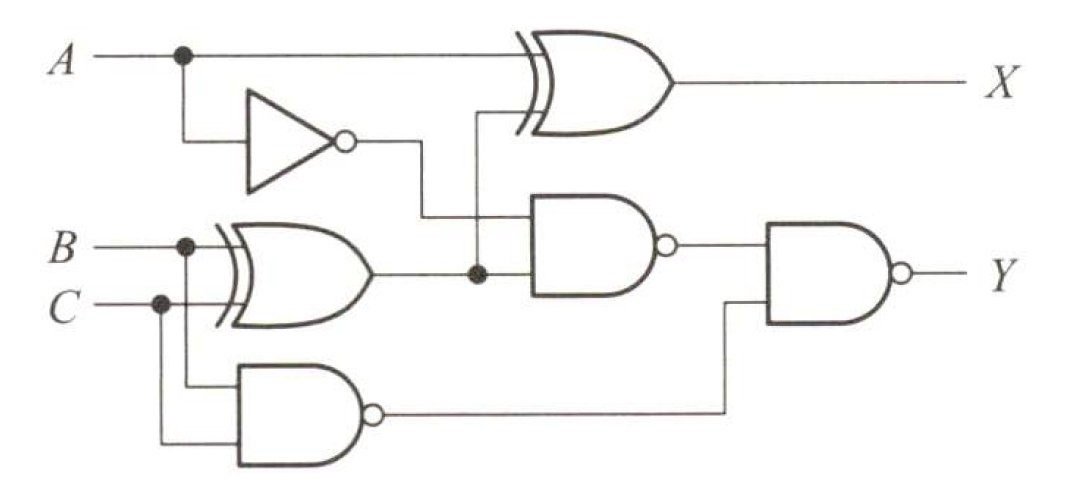
\includegraphics[scale=0.2]{SD4.1.5}
	\caption{4.1.5}
\end{figure}
解:
\textbf{4.1.6} 分析图题4.1.6所示逻辑电路的功能\\
\begin{figure}[H]
	\centering
	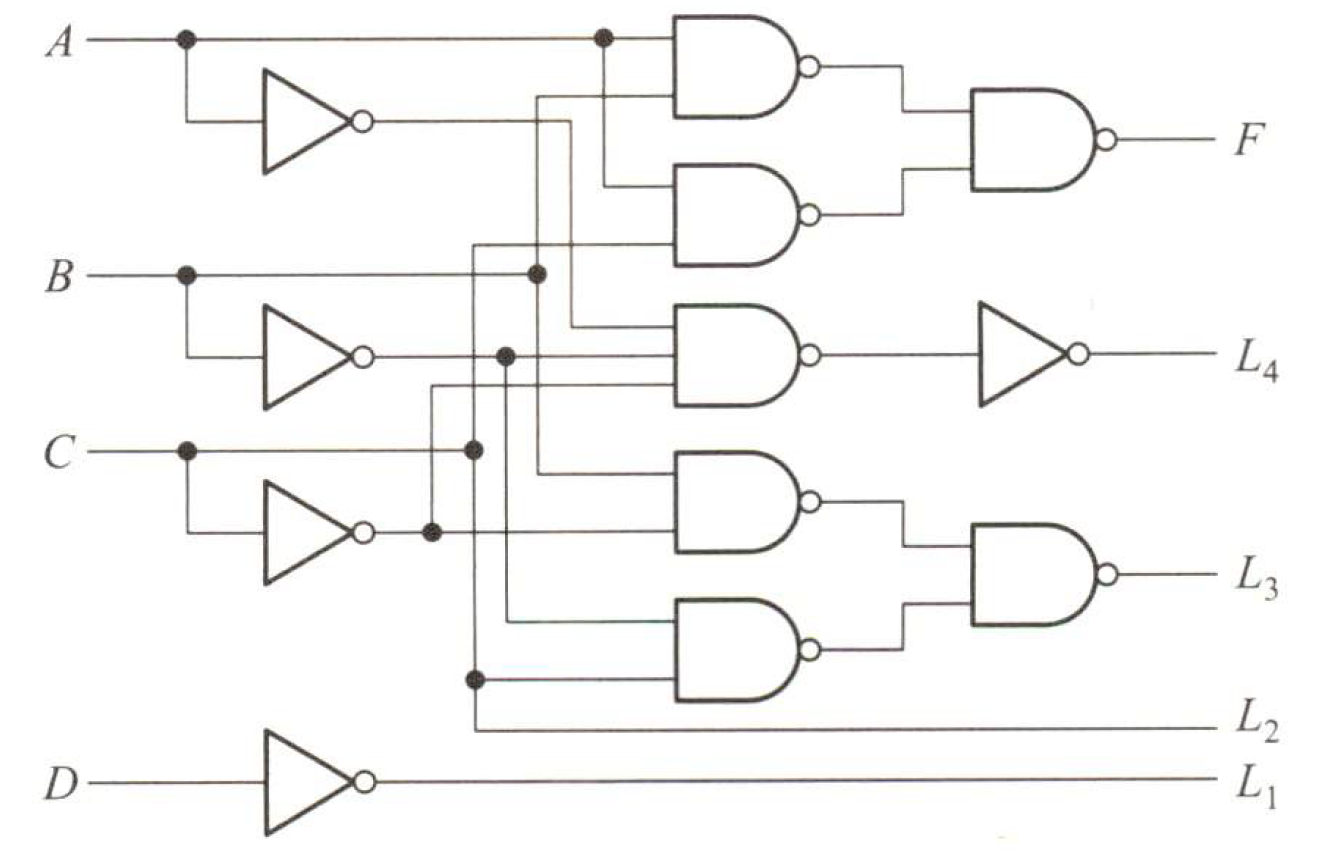
\includegraphics[scale=0.15]{SD4.1.6}
	\caption{4.1.6}
\end{figure}
\textbf{4.2.9} 某足球评委会由一位教练和三位球迷组成,对裁判员的判罚进行比爱绝。当满足一下条件时表示同意:有三人或三人以上同意,或者两人同意,但其中有一人是教练。试用2输入\textbf{与非}门设计该表决电路(写出完整的设计流程,以及Verilog HDL程序)\\
\textbf{4.2.11} 某火车站有特快、直快和慢车三种类型的客运列车进出,试用2输入与非门和反相器设计一个指示列车等待进展的逻辑电路,3个指示灯一、二、三号分别对应特快、直快、慢车。列车的优先级别依次为特快、直快、慢车,要求当特快列车请求进站时无论其他两种列车是否请求进站,一号灯亮。当特快没有请求,直快请求进站时,无论慢车是否请求,二号灯亮,当特快和直快均没有请求,而慢车有请求时,三号灯亮。(写出完整的设计流程,以及Verilog HDL程序)\\
\textbf{4.2.12} 会议室顶灯分别有安装在4扇门旁边的4个开关控制,设计一个控制电路,要求改变任意一个开关的状态都能打开或关闭顶灯,可以采用任何门电路来实现(写出完整的设计流程,以及Verilog HDL程序)\\
\textbf{4.2.13} 某化工厂有5种原料,编号为1到5,在使用时必须遵守以下规则:\\
(1)用第3号时必须使用第1号。\\
(2)第2号和第4号必须同时使用。\\
(3)第2号和第5号不能同时使用。\\
试设计一个逻辑电路,能在违反上述任何一项规定时给出高电平知识信号。写出逻辑表达式。(直接写出表达式并化简,无需Verilog HDL)\\
\textbf{4.2.15} 设计一2为二进制数相加的逻辑电路,可以用任何门电路实现,化简变换时考虑多输出函数的公共乘积项,以减少门的数目。(写出完整设计流程,无需Verilog HDL)\\
\end{document}